% !TEX root = main.tex
\section{The experiment}
In this section we now describe the experiments we conducted.
We first present the general set-up of the experiments, then we will describe how we defined the base cases for each experiments in order to perform tests against them.
After that we will go through the deception techniques we used to deceive the users in order to avoid bias in the results, and finally we will describe in detail the specific experiments. 

\subsection{Testers}
The testers were graduate and undergraduate students, whose participation was completely voluntary. In order to incentivize them we offered a small candy as a reward.

\subsection{Set up}
The testers interacted with an iPad application in which they are told to perform actions on a balloon on the screen. The iPad choice has been determined by the will of keeping the interaction as natural as possible in order not to make it influent over the measurement of the synchronization aspects of the experiments; the touch interaction on an iPad screen seemed to be the most suitable choice.
The testers were sit on a desk in a quiet room, with wearing headphones while interacting with the iPad applications.
The approximate duration of the tests per each user was about 5 minutes.

\subsection{Deception}
Due to the configuration discussed above, there could have been the risk that a tester would have understood the purpose of the test. In fact she could have got the purpose of the test noticing that we were enforcing her to wear headphones. This could have brough some bias in the data collection as the tester could have voluntarily tried to synchronize with the soundtrack.
We then try to deceive her bye the explaining the presence of the headphones as way to increase the concentration on the task, avoiding outside interference.

\subsection{Base cases}
\label{sec:base-cases}
We are clearly interested to the effects the background tempo produces on the participants, therefore both of the experiment run with a background music we chose.
Since we wanted to see whether there is a synchronization between the background tempo and the actions the user is performing, we first of all set a base case for all the experiments. By base case we mean a test run of the experiments \emph{without} music across multiple users, in order to determine an average measure for each experiment (we will discuss about the measures later in Section~\ref{sec:measures}).

\subsection{\testfirst}
\label{sec:test1}
The first test consisted of an application where the user was asked to tap a red balloon present on the screen. In Figure~\ref{fig:test1} is shown an in-game screen shot of the application.

Every time the user tapped on the balloon, this instantaneously moved to a different random location on the screen. The result of such an interaction is the user chasing the balloon around the screen, repeatedly tapping on it. This went on for 45 seconds.
The whole sequence is sent in real time to a web-server we developed and stored on a remote database for further analysis.

It's worthy of notice the fact that in this experiment the user had no specific goal if not the one of pressing the button. Moreover they were not aware of the duration of the experiment.

This represents a significant difference w.r.t. the second experiment (presented in Section~\ref{sec:test2}), as we will discuss later on.

Another significant difference of our interest is that this task requires a non trivial cognitive activity: the user has to be focused on the game in order to follow the balloon movements.
\todo[inline]{Say something about whether this makes any difference after we have the results}

\begin{figure}[h!t]
\label{fig:test1}
\centering
	{\setlength{\fboxsep}{0pt}
	 \fbox{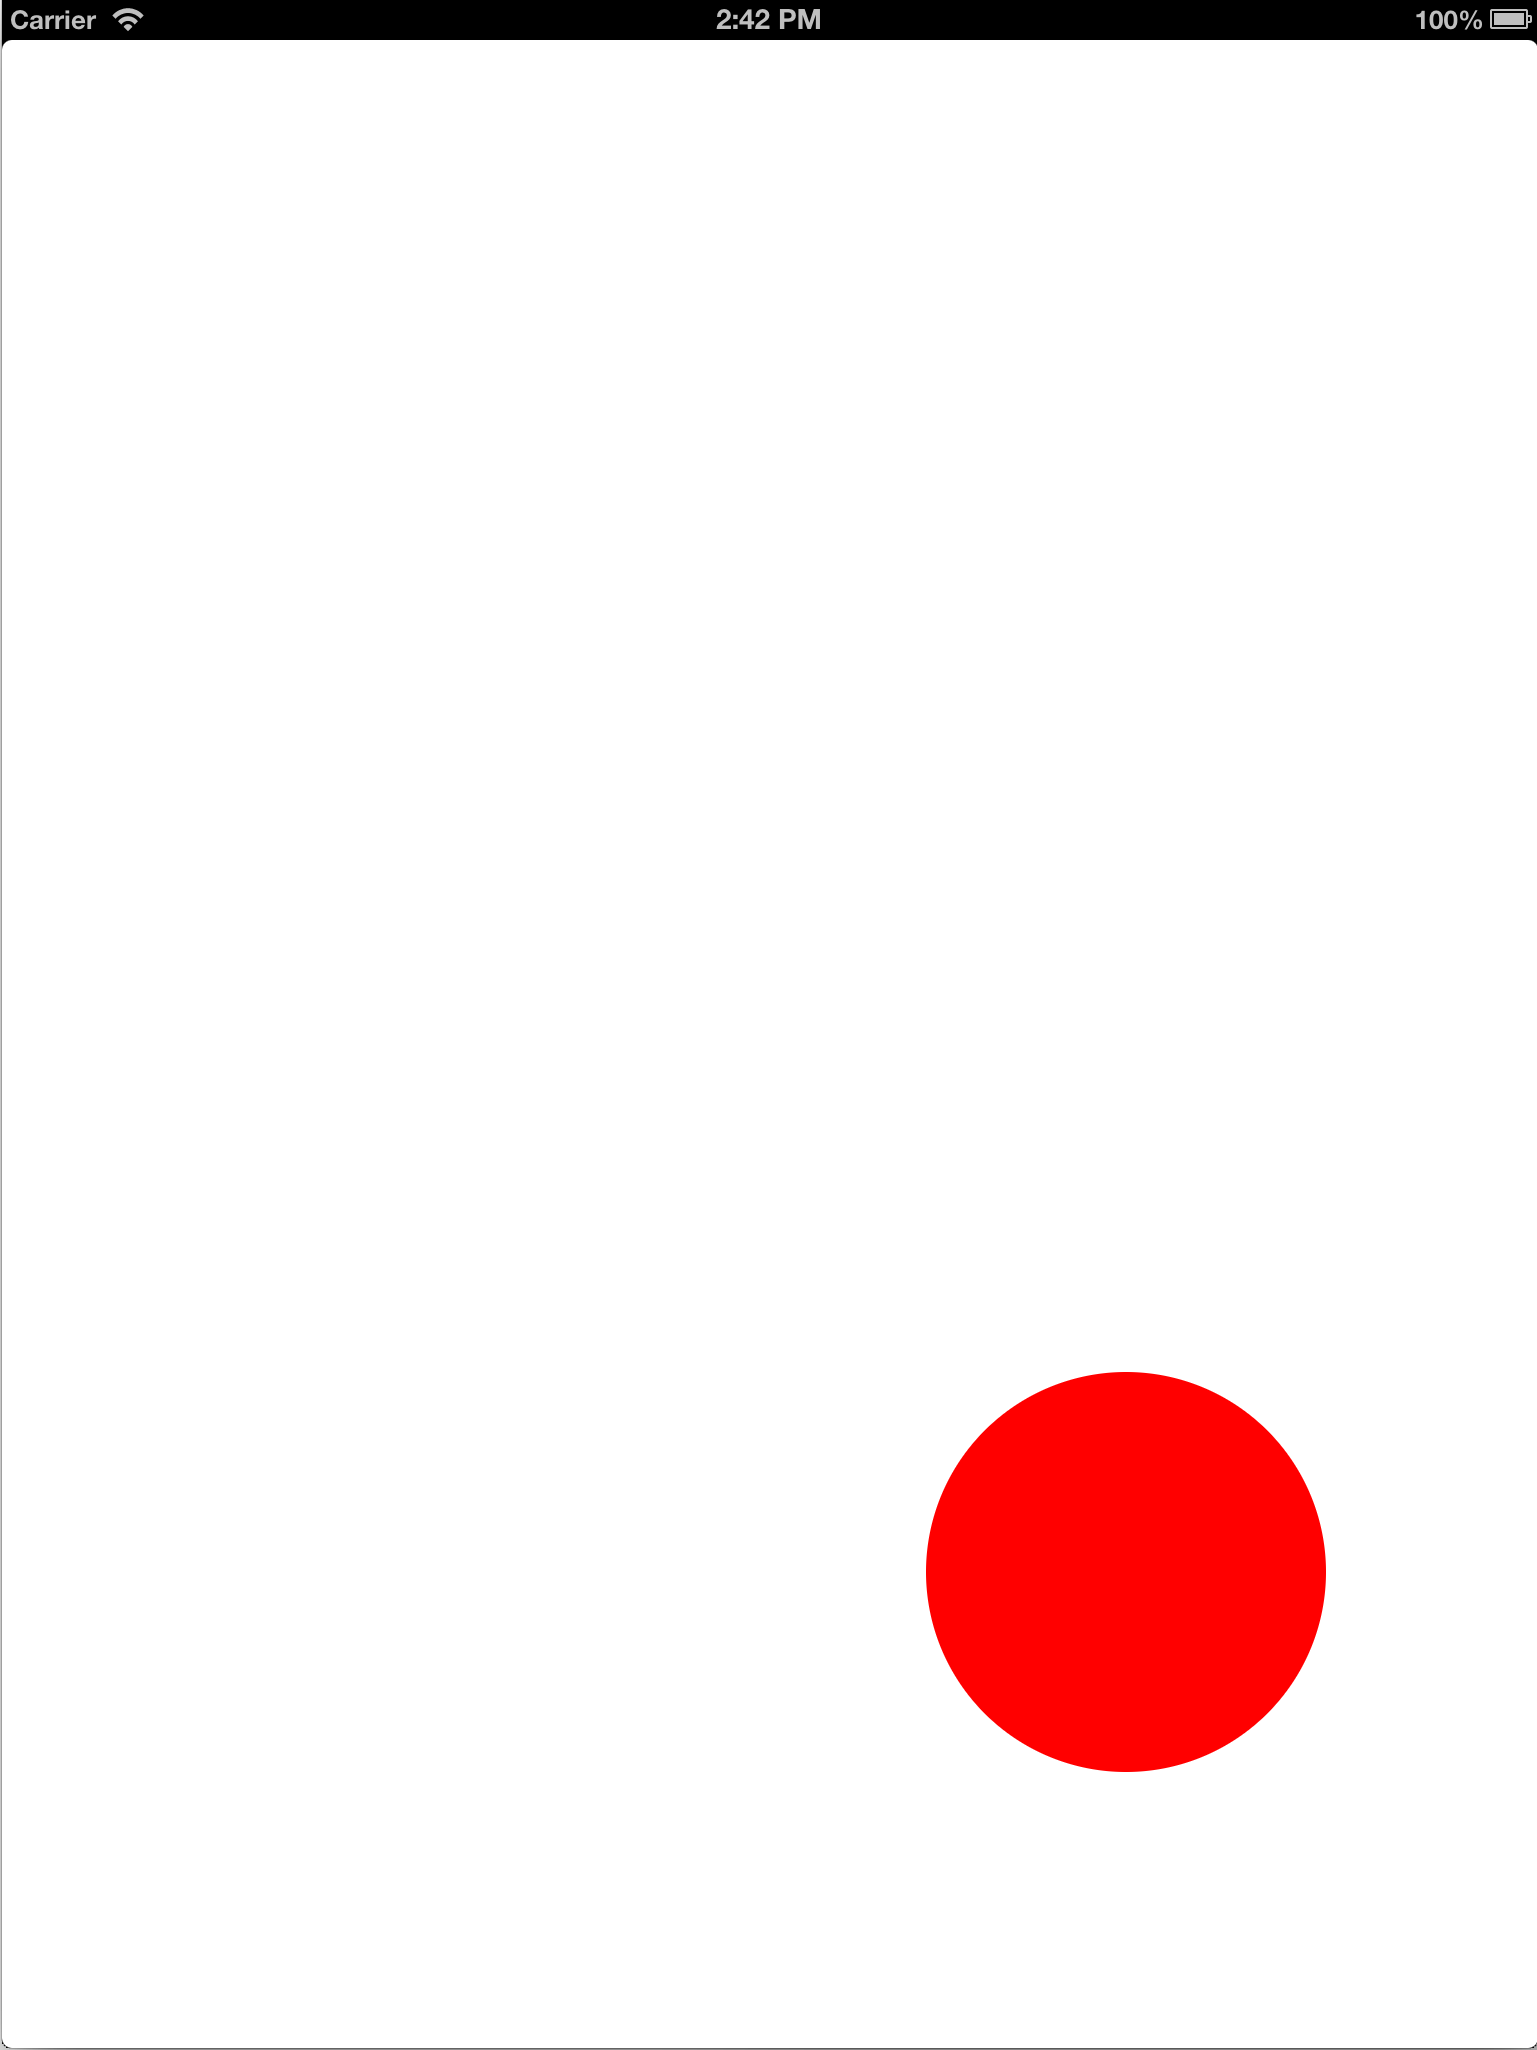
\includegraphics[width=0.45\textwidth]{test1}}}
\caption{\testfirst: in-game screenshot}
\end{figure}

\subsection{Balloon inflater}
\label{sec:test2}
The second test consisted of an application where the user was asked to inflate a balloon on the screen by tapping on it.
The balloon enlarged at every tap and shrank if not touched.
The resulting interaction is the user tapping repeatedly on the balloon in order to make it bigger, with the final result of making it explode as its dimension went beyond the screen bounds.

With respect to the previous test the interaction required much less cognitive activity, in the sense that the user concentration on the screen was not required in order to achieve the final result of exploding the balloon.

Moreover this second test had a clear goal -- inflating the balloon -- whereas the first one, as stated before, had not.

We will discusses later in Section~\ref{sec:results} how this differences impacted on the test results.
\todo[inline]{Come back on this after we have the results}

\missingfigure{The second test}
